\usetikzlibrary{angles}
\begin{center}
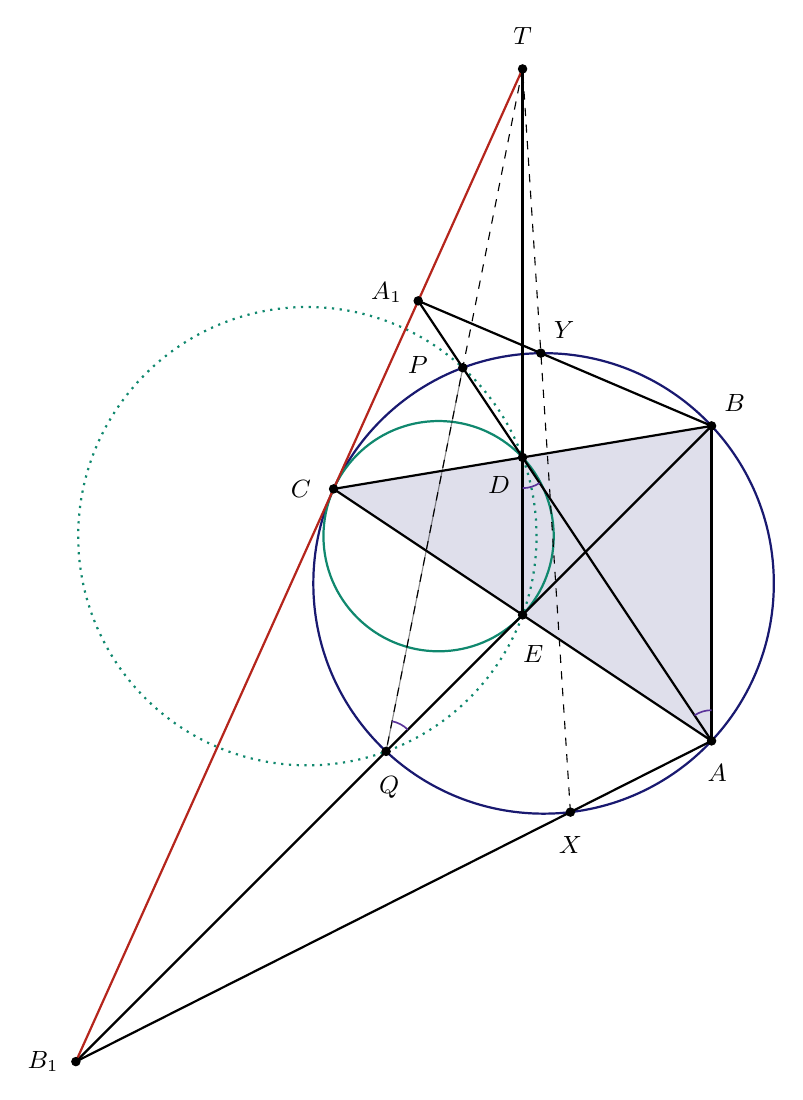
\begin{tikzpicture}[scale=0.8, font=\small]
    \fill[fill=MidnightBlue, fill opacity=0.14] (0, 0)--(0, 5)--(-6, 4)--cycle;
    \coordinate (A) at (0, 0);
    \path (A) ++(0.09, -0.512) node[inner sep=0pt] {$A$};
    \coordinate (B) at (0, 5);
    \path (B) ++(0.368, 0.368) node[inner sep=0pt] {$B$};
    \coordinate (C) at (-6, 4);
    \path (C) ++(-0.52, 0) node[inner sep=0pt] {$C$};
    \coordinate (D) at (-3, 4.5);
    \path (D) ++(-0.373, -0.444) node[inner sep=0pt] {$D$};
    \coordinate (E) at (-3, 2);
    \path (E) ++(0.168, -0.628) node[inner sep=0pt] {$E$};
    \coordinate (A1) at (-4.65672, 6.98507);
    \path (A1) ++(-0.502, 0.135) node[inner sep=0pt] {$A_{1}$};
    \coordinate (B1) at (-10.09091, -5.09091);
    \path (B1) ++(-0.52, 0) node[inner sep=0pt] {$B_{1}$};
    \coordinate (T) at (-3, 10.66667);
    \path (T) ++(0, 0.52) node[inner sep=0pt] {$T$};
    \coordinate (P) at (-3.94872, 5.92308);
    \path (P) ++(-0.715, 0.04) node[inner sep=0pt] {$P$};
    \coordinate (Q) at (-5.16667, -0.16667);
    \path (Q) ++(0.051, -0.578) node[inner sep=0pt] {$Q$};
    \coordinate (X) at (-2.24054, -1.13036);
    \path (X) ++(0, -0.52) node[inner sep=0pt] {$X$};
    \coordinate (Y) at (-2.70955, 6.15503);
    \path (Y) ++(0.368, 0.368) node[inner sep=0pt] {$Y$};

    \draw[thick, MidnightBlue] (-2.66667, 2.5) circle (3.65529);
    \draw[thick, PineGreen, dotted] (-6.41667, 3.25) circle (3.63815);
    \draw[thick, PineGreen] (-4.33333, 3.25) circle (1.82764);
    \draw[thick] (A)--(B);
    \draw[thick] (B)--(C);
    \draw[thick] (C)--(A);
    \draw[thick] (A)--(A1);
    \draw[thick] (B)--(B1);
    \draw[thick, BrickRed] (B1)--(T);
    \draw[thin, dashed] (X)--(T);
    \draw[thin, dashed] (T)--(Q);
    \draw[thick] (E)--(T);
    \draw[thick] (B1)--(A);
    \draw[thick] (B)--(A1);
    \draw[thin, opacity=0.45] (Q)--(P);
    \pic[draw=RoyalPurple, semithick, angle radius=0.39cm] {angle=E--Q--P};
    \pic[draw=RoyalPurple, semithick, angle radius=0.39cm] {angle=E--D--A};
    \pic[draw=RoyalPurple, semithick, angle radius=0.39cm] {angle=B--A--D};

    % Radius cetak titik tetap 1.5pt saat scale diubah.
    \pgfgettransformentries{\studioXX}{\studioYX}{\studioXY}{\studioYY}{\studioDX}{\studioDY}
    \pgfmathsetlengthmacro{\studioRadiusTitik}{1.5pt/veclen(\studioXX,\studioYX)}
    \foreach \s in {A,B,C,D,E,A1,B1,T,P,Q,X,Y}
        \filldraw (\s) circle (\studioRadiusTitik);
\end{tikzpicture}
\end{center}
